\section{Qualità software}
\label{sec:qualita_software}

Con \strong{qualità} si intende l'insieme delle caratteristiche di un'entità che
ne determinano la capacità di soffisfare esigenze espresse e implicite.

Vi sono diverse visioni, o punti di vista, da cui valutare la qualità, e su cui
il sistema qualità agisce:

\begin{itemize}
  \item Intrinseca: conformità ai requisiti, idoneità all'uso;
  \item Relativa: soddisfazione del cliente;
  \item Quantitativa: misura del livello di qualità per confronto;
\end{itemize}

Secondo ISO/IEC 9001, per \strong{qualità software} si intende la ``capacità di
un prodotto software di soddisfare i requisiti.'' Vi sono però due aspetti della
qualità: uno riguarda considerazioni oggettive, indipendenti dall'uomo, mentre
l'altro ha a che fare con l'esperienza dell'utente con quel prodotto, come
risultato delle caratteristiche oggettive. La qualità software non riguarda
quindi solamente il livello di aderenza ai requisiti (aspetti funzionali), ma
dipende principalmente dai suoi attributi non funzionali.

\subsection{Sistema di qualiltà}
\label{sub:sistema_di_qualilta}

Con \strong{sistema qualità} si identifica la struttura organizzativa, i
processi e le risorse messe in atto per il perseguimento della qualità.

\subsubsection{Documentazione del SGQ}
\label{ssub:documentazione_del_sgq}

La normativa prevede della documentazione per la realizzazione del SGQ, tra cui
un Manuale della Qualità e un Piano della Qualità.

Il \strong{Manuale della Qualità} è il documento che definisce il sistema di
gestione della Qualità di un'organizzazione. Esprime una visione orizzontale (a
livello aziendale) e ad alto livello, integrandosi con le procedure aziendali e
fissando obiettivi di qualità e strategie attuative. Il Manuale di Qualità
esprime le \strong{politiche aziendali} rispetto alla qualità.

Il \strong{Piano della Qualità} è il documento che definisce gli elementi del
SGQ e le risorse che devono essere applicate in uno \strong{specifico caso}
(prodotto, processo, progetto). Rappresenta una visione strategica, verticale;
concretizza il Manuale della Qualità a livello di progetto, quindi sotto
specifici vincoli di tempo e risorse.

Il Piano di Qualità, accerta la disponibilità di analisi dei requisiti,
pianificazione e, risultati delle verifiche e delle prove, nonchè la
tracciabilità di soluzioni e requisiti.

\subsubsection{Gestione della qualità}
\label{gestione_della_qualita}

Con \strong{gestione della qualità} si intendono le attività del sistema qualità
pianificate e attuate affinchè prodotti, servizi e processi soddisfino i
requisiti di qualità. Comprende le attività di pianificazione della qualità,
\frgnword{quality assurance}, controllo della qualità e miglioramento di
processo.

\begin{itemize}
  \item \strong{Pianificazione di qualità}: definisce gli obiettivi di qualità,
    e i processi e le risorse necessarie per conseguirli. I risultati della
    pianificazione sono raccolti nel Piano di Qualità, che descrive le
    caratteristiche di qualità desiderate per il software, e come queste devono
    essere valutate;
  \item \strong{\frgnword{Quality assurance}}:
    Rappresenta la sistematica misurazione, confronto e monitoraggio dei
    processi, con l'obbiettivo di prevenzione dell'errore. È in contrasto con il
    controllo della qualità, che pone l'attenzione sulle uscite dei processi;
  \item \strong{Controllo della qualità}: attività che esaminano specifici
    prodotti di progetto per determinare la loro conformità verso gli standard
    di qualità scelti; i prodotti sono esaminati durante tutta la durata del
    progetto, in punti strategici di avanzamento;
  \item \strong{Miglioramento dei processi}: attività che cercano di migliorare
    l'efficacia e l'efficienza dei processi, con l'obbiettivo ultimo di
    migliorare la qualità del prodotto software.
\end{itemize}

\subsection{Standard di qualità}

Gli standard di qualità giocano un ruolo molto importante nella gestione della
qualità del software. Essi:

\begin{itemize}
  \item Catturano e rappresentano le conoscenze, l'\strong{esperienza} e le
    \frgnword{best-practice};
  \item Supportano la \strong{continuità} nel momento in cui il lavoro svolto da
  una
    persona viene continuato da un'altra: processi standardizzati sono
    facilmente comprensibili da nuovi assunti;
\end{itemize}

Un uso errato degli standard può avere effetti negativi. E' importante che le
norme siano snelle, chiaramente complensibili e supportabili da strumenti
automatizzati.

\begin{itemize}
  \item Se gli standard sono poco comprensibili, il personale può percepirli
    come irrilevanti o bloccanti;
  \item La loro attuazione cieca può comportare eccessi di burocrazia;
  \item Senza il supporto di strumenti informatici, possono richiedere tediose
    attività manuali;
\end{itemize}

\paragraph{Definizione e valutazione di qualità}
\label{par:definizione_e_valutazione_di_qualita}

Gli standard forniscono inoltre modelli e metriche per la \strong{definizione} e
la \strong{valutazione} della qualità del software, eliminando le percezioni
soggettive e convertendo proprietà astratte e poco chiare in valori
quantificabili e misurabili.

\begin{itemize}
  \item \strong{Definizione: modello di qualità}: catalogazione sistematica
    delle caratteristiche rilevanti;
  \item \strong{Valutazione: metriche}: definizione di metriche per la
    valutazione delle caratteristiche di qualità.
\end{itemize}

Un esempio di standard di qualità è l'ISO/IEC 9126.

\subsubsection{Definizione della qualità: modelli di qualità software}

I modelli di qualità classificano la qualità software in un insieme strutturato
di \strong{caratteristiche} (suddivise ulteriormente in attributi), e
costituiscono un modello unico e comune per committenti e fornitori,
\strong{uniformando} la percezione e la valutazione della qualità. Il Piano di
Qualità è il documento che definisce quali di questi attributi sono ritenuti più
importanti per un determinato prodotto.

Esempi di modelli di qualità sono il modello di Bohem e l'ISO/IEC 9126:2001.

\begin{figure}[h]
  \centering
  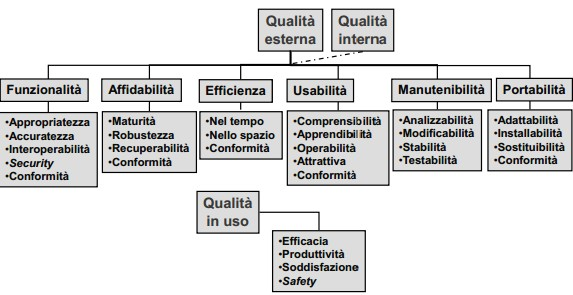
\includegraphics[scale=0.6]{imgs/isoiec_9126_2001.jpg}
  \caption{Caratteristiche di qualità software secondo il modello
    ISO/IEC9126:2001}
\end{figure}

I modelli di qualità definiscono valutazioni di qualità secondo più punti di
vista:

\begin{itemize}
  \item Visione dell'\strong{utente}, rispetto all'utilizzo pratico;
  \item Visione della \strong{produzione}, rispetto a qualifica, manutenzione,
    portabilità e riuso;
  \item Visione della \strong{direzione}, rispetto al rapporto costi/benefici;
\end{itemize}

\subsubsection{Valutazione della qualità: metriche}

Con valutazione della qualità intendiamo il processo attraverso cui, con l'uso
di metriche definite, vengono assegnati valori ad attributi di una entità su una
scala predefinita.

Definiamo \strong{metrica} qualsiasi tipo di misurazione riguardante un sistema,
un processo o un documento software. Le metriche costituiscono uno
\strong{strumento di quantificazione} del prodotto e del processo.

\paragraph{Attributi interni e esterni}

Le metriche misurano attributi di qualità interni del sistema, ma spesso siamo
più interessati a quelli esterni. Questi attributi, come mantenibilità o
usabilità, sono tipicamente difficili da misurare, poichè dipendono da fattori
soggettivi relativi all'esperienza dell'utente. Per farlo, occorre misurare gli
attributi interni e assumere che esista una relazione con gli attributi esterni
che si vogliono valutare.

Perchè la misurazione di un attributo interno del software sia utile alla
valutazione di una caratteristica esterna, occorre che

\begin{enumerate}
  \item L'attributo interno sia misurato correttamente;
  \item Il valore dell'attributo di qualità sia, in qualche modo, correlato con
    il valore che si sa misurare;
  \item La relazione sia esprimibile e validabile formalmente in termini di
    formula o modello.
\end{enumerate}

\begin{figure}[h]
  \centering
  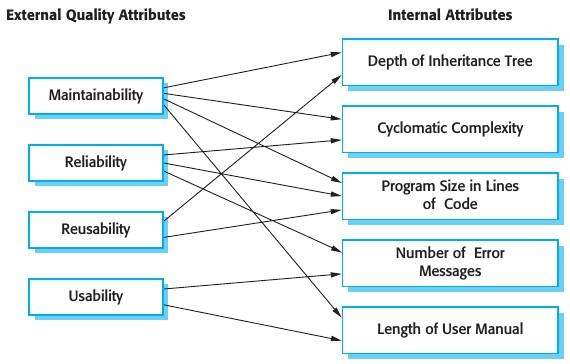
\includegraphics[scale=0.6]{imgs/int_ext_attrib.jpg}
  \caption{Relazione tra caratteristiche esterne e attributi interni del
    software}
\end{figure}

\subsubsection{ISO 9000}
\label{ssub:iso_9000}

ISO 9000 è una famiglia di standard di qualità, con l'obbiettivo di integrare un
sistema di qualità in azienda. Esso suddivide i processi in quattro categorie:

\begin{itemize}
  \item Responsabilità della direzione;
  \item Gestione delle risorse;
  \item Realizzazione del prodotto;
  \item Misura, analisi e miglioramento.
\end{itemize}

\subsection{Qualità di processo}
\label{sub:qualita_di_processo}

La qualità di un prodotto è direttamente collegata alla qualità del processo
impiegato per crearlo. Per ottenere qualità di processo, è necessario

\begin{itemize}
  \item \strong{Definire} il processo, per poterlo facilmente controllare;
  \item \strong{Controllare} il processo, per migliorarne efficienza ed
    efficacia;
  \item Usare buoni strumenti di \strong{valutazione}.
\end{itemize}

Tecniche quali il ciclo di Deming offrono metodi per specificare obbiettivi di
qualità e verificarne l'effettivo raggiungimento.

\subsubsection{Strumenti di valutazione dei processi}
\label{ssub:strumenti_di_valutazione}

\begin{itemize}
  \item Software Process Assessment \& Improvement (SPY): valutazione oggettiva
    dei processi di una organizzazione, per darne un giudizio di maturità e
    individuare azioni migliorative;
  \item Capability Maturity Model Integration (CMMI): modello per la
    valutazioine uniforme dei fornitori;
  \item Software Process Improvement Capability dEtermination (SPICE): nato per
    armonizzare SPY con ISO/IEC 12207 e ISO 9001.
\end{itemize}

\par{Capability and Maturity Model Integration (CMMI)}
\label{par:capability_and_maturity_model_integration}

CMMI è un insieme strutturato di elementi che descrivono le caratteristiche di
processi efficaci. Costituisce una base concettuale su cui appoggiarsi per la
valutazione e il miglioramento dei processi, costruita su best-practice, e un
riferimento per valutare il miglioramento di un'azienda o confrontarne di
diverse.

\begin{itemize}
  \item \strong{Capability}: misura di quando un processo, considerato
    singolarmente, è adeguato in termini di efficienza ed efficacia;
  \item \strong{Maturity}: quanto il sistema dei processi dell'azienda è
    governato;
  \item \strong{Model}: insieme di requisiti di qualità per valutare il percorso
    di miglioramento;
  \item \strong{Integration}: architettura di integrazione delle diverse
    attività aziendali.
\end{itemize}

\begin{figure}[h!]
  \centering
  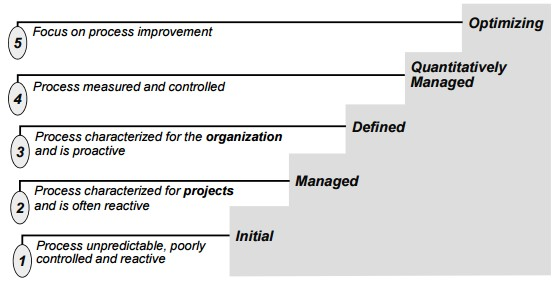
\includegraphics[scale=0.5]{imgs/cmmi_maturity_level}
  \caption{Livelli di maturità di CMMI}
\end{figure}

\par{ISO/IEC 15504 (SPICE)}
\label{par:spice}

ISO/IEC 15504, \frgnword{aka} SPICE, è un modello di riferimento per modelli di
maturità, utilizzando il quale si può valutare il livello generale di maturità
dell'azienda.

Il modello di riferimento definisce una \strong{dimensione di processo} e una
\strong{dimensione di capacità} (\frgnword{capability}).

La dimensione di processo divide i processi in cinque categorie:

\begin{itemize}
  \item Customer supplier;
  \item Engineering;
  \item Supporting;
  \item Management;
  \item Organization.
\end{itemize}

Per ogni processo, lo standard definisce un livello di capacità
(\frgnword{capability level}) sulla seguente scala:

\begin{enumerate}
  \item[0] Incomplete process;
  \item[1] Performed process;
  \item[2] Managed process;
  \item[3] Established process;
  \item[4] Predictable process;
  \item[5] Optimizing process.
\end{enumerate}

Lo standard specifica nove attributi di processo utilizzati per valutare la
capacità di processo, oltre che una metodologia di valutazione, che si compone
delle seguenti operazioni:

\begin{enumerate}
  \item Identificazione dei portatori d'interesse: i destinatari dei
    risultati e i responsabili dei processi valutati e delle attività di
    valutazione;
  \item Scelta tra valutazione e miglioramento: risultato a uso interno o
    esterno, valutazione formale o meno;
  \item Definizione della portata: processi inclusi nella valutazione,
    indicatori di valutazione.
\end{enumerate}
